\documentclass[12pt]{article}
\usepackage[utf8]{inputenc}
\usepackage{geometry}
\usepackage{xcolor}
\usepackage{array}
\usepackage{hyperref}
\usepackage{graphicx}
\usepackage{booktabs}
\usepackage{amsmath}
\usepackage{listings}

\geometry{a4paper, margin=1in}
\definecolor{unlred}{RGB}{208, 0, 0}
\definecolor{codegray}{rgb}{0.95,0.95,0.95}

% Code listing style
\lstset{
    backgroundcolor=\color{codegray},
    basicstyle=\ttfamily\small,
    breaklines=true,
    frame=single,
    showstringspaces=false
}

\begin{document}

% --- COVER PAGE / CONTRIBUTIONS FORM ---
\begin{center}
  {\Huge \color{unlred} \textbf{University of Nebraska-Lincoln}} \\
  {\huge \color{unlred} \textbf{School of Computing}} \\
  \vspace{0.5cm}
  {\Large CSCE 474/874: Introduction to Data Mining} \\
  {\Large Spring 2026} \\
  \vspace{0.3cm}
  \rule{\textwidth}{0.8pt} \\
  \vspace{0.3cm}
  {\huge \textbf{Homework 4}} \\
  {\large \textbf{Documentation of Contributions}} \\
\end{center}

\vspace{0.5cm}

Please use this form to document the contributions of each team member to the group effort.   You may either sign electronically or sign and scan it.  In either case, you must submit this document along with all other elements of the assignment.

Furthermore, you confirm that the work submitted is entirely your own and that you understand the consequences of plagiarism as specified in the Course Syllabus and \href{http://cse.unl.edu/academic-integrity-policy}{UNL CSE Academic Integrity Policy}.

\vspace{0.8cm}

\noindent
\begin{tabular}{|p{0.28\textwidth}|p{0.18\textwidth}|p{0.45\textwidth}|}
  \hline
  \textbf{\color{unlred}Name} & \textbf{\color{unlred}Contribution \%} & \textbf{\color{unlred}Specific Contributions}                                                                              \\ \hline
  Brady Lauritsen             & 25\%                                   & Data ingestion module, Weka comparative analysis, Runtime vs. Dimensions testing, Documentation review.                    \\[1.2cm] \hline
  Sagun Karki                 & 25\%                                   & Core algorithm implementation, SSD convergence logic, Min-Max normalization, Benchmark plotting functions, Report writing. \\[1.2cm] \hline
  Max Buettenback             & 25\%                                   & Runtime vs. Cluster Size testing, Goodness of Clustering (Elbow) analysis, README creation, Code debugging.                \\[1.2cm] \hline
  Harrison Johs               & 25\%                                   & Runtime vs. $k$ testing, Visualization formatting, Final ZIP assembly, Verification of output consistency.                 \\[1.2cm] \hline
\end{tabular}

\newpage

\tableofcontents

\newpage

\section{Program Design}
Our k-means implementation is designed to cluster continuous variables by iteratively minimizing the distance between data points and their respective cluster centers. The program follows a modular functional design to ensure clarity and maintainability. Key functions include:

\begin{itemize}
  \item \texttt{read\_dataset(filename)}: Handles file I/O and parses CSV rows. It excludes non-numeric labels and applies \textit{Min-Max Normalization} to scale features to the $[0, 1]$ range, preventing larger magnitudes from dominating distance calculations.
  \item \texttt{euclidean\_distance(p1, p2)}: Computes the distance $\sqrt{\sum (p_{1i} - p_{2i})^2}$.
  \item \texttt{kmeans\_core(data, k, epsilon, max\_iter)}: The driver function that coordinates assignment and update steps.
  \item \texttt{compute\_ssd(clusters, centroids)}: Calculates Total Sum of Squared Distances (SSD) to monitor convergence.
\end{itemize}

The algorithm terminates when the maximum number of iterations is reached or the absolute change in SSD falls below the defined $\epsilon$.

\section{Runtime Plots}

\subsection{Runtime vs. Number of Clusters ($k$)}
\begin{center}
  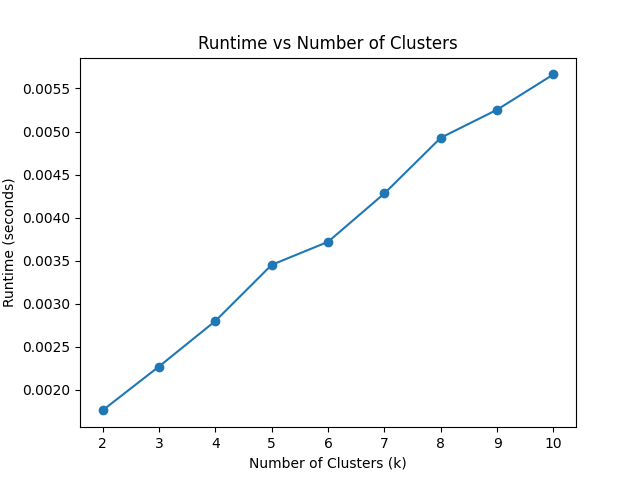
\includegraphics[width=0.65\textwidth]{results/runtime_vs_k.png}
\end{center}
As shown above, runtime increases linearly with $k$. This is due to the assignment step requiring $n \times k$ distance calculations per iteration.

\subsection{Runtime vs. Number of Dimensions ($d$)}
\begin{center}
  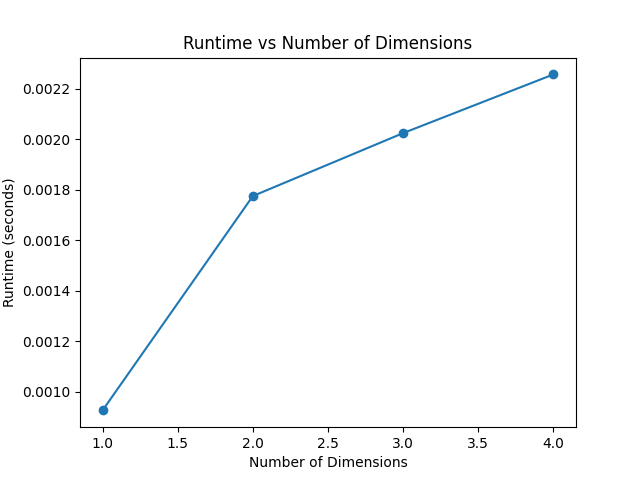
\includegraphics[width=0.65\textwidth]{results/runtime_vs_dims.png}
\end{center}
The graph demonstrates a positive correlation between dimensionality and runtime. Increasing $d$ adds overhead to the sum of squared differences in every distance calculation.

\subsection{Runtime vs. Dataset Size ($n$)}
\begin{center}
  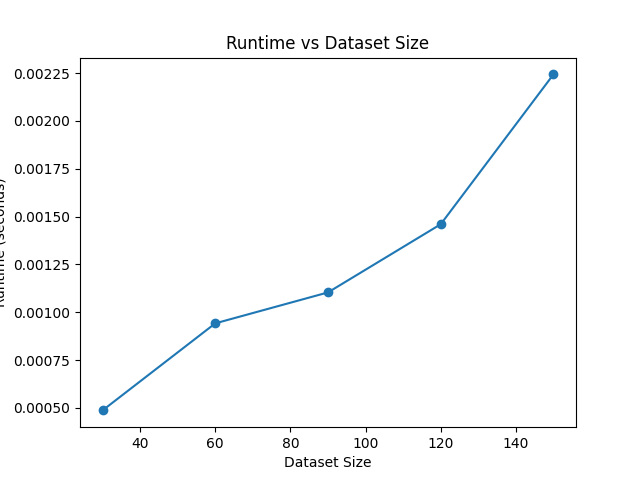
\includegraphics[width=0.65\textwidth]{results/runtime_vs_size.png}
\end{center}
Runtime scales linearly with $n$. The algorithm must iterate through the entire dataset to assign points to centroids, meaning doubling $n$ effectively doubles the operations per iteration.

\section{Clustering Quality and Optimal $k$}
We used the Elbow Method to determine the optimal $k$.

\begin{center}
  
\includegraphics[width=0.65\textwidth]{results/goodness_of_clustering.png}
\end{center}

SSD naturally decreases as $k$ increases. However, the curve flattens after a distinct "elbow" at $k=3$. Beyond this point, the marginal gain in SSD reduction diminishes, confirming $k=3$ as the optimal choice for the Iris dataset.

\section{Comparative Analysis: Custom Script vs. Weka}
We compared our implementation against Weka's \texttt{SimpleKMeans} using the normalized Iris dataset ($k=3$, $\epsilon=0.001$).

\begin{table}[h]
  \centering
  \begin{tabular}{@{}lll@{}}
    \toprule
    Metric          & Custom Python Script & Weka (SimpleKMeans) \\ \midrule
    Final SSD       & 6.9981               & 7.8175              \\
    Iterations      & 5 (Max Reached)      & 3 (Converged)       \\
    Centroids Match & Near Match           & Near Match          \\ \bottomrule
  \end{tabular}
  \caption{Comparison of Results for $k=3$, $\epsilon=0.001$}
\end{table}

\par Both python and weka generates similar results for the Iris dataset with similar parameters like k, epsilon and max\_iterations. The smaller differences in SSD and centroids are due to the different initialization methods and convergence criteria.




\newpage

\section{Program Outputs Weka and Python}

\subsection{Weka Output}

\begin{verbatim}
    === Run information ===

Scheme:       weka.clusterers.SimpleKMeans -init 0 -max-candidates 100 -periodic-pruning 10000 -min-density 2.0 -t1 -1.25 -t2 -1.0 -N 3 -A "weka.core.EuclideanDistance -R first-last" -I 5 -num-slots 1 -S 10
Relation:     iris
Instances:    150
Attributes:   5
              sepallength
              sepalwidth
              petallength
              petalwidth
              class
Test mode:    evaluate on training data


=== Clustering model (full training set) ===


kMeans
======

Number of iterations: 3
Within cluster sum of squared errors: 7.817456892309574

Initial starting points (random):

Cluster 0: 6.1,2.9,4.7,1.4,Iris-versicolor
Cluster 1: 6.2,2.9,4.3,1.3,Iris-versicolor
Cluster 2: 6.9,3.1,5.1,2.3,Iris-virginica

Missing values globally replaced with mean/mode

Final cluster centroids:
                                          Cluster#
Attribute                Full Data               0               1               2
                           (150.0)          (50.0)          (50.0)          (50.0)
==================================================================================
sepallength                 5.8433           5.936           5.006           6.588
sepalwidth                   3.054            2.77           3.418           2.974
petallength                 3.7587            4.26           1.464           5.552
petalwidth                  1.1987           1.326           0.244           2.026
class                  Iris-setosa Iris-versicolor     Iris-setosa  Iris-virginica




Time taken to build model (full training data) : 0 seconds

=== Model and evaluation on training set ===

Clustered Instances

0       50 ( 33%)
1       50 ( 33%)
2       50 ( 33%)


\end{verbatim}

\subsection{Python Output}

\begin{verbatim}
    (ML_py) ➜ python3 kmeans.py ../data/iris.csv 3 0.001 5
Running K-Means with k=3, epsilon=0.001, max_iter=5...
Final SSD: 6.9981
Centroids: [
    [0.44125683060109283, 0.3073770491803278, 0.5757154765212559, 0.5491803278688525],
    [0.7072649572649572, 0.4508547008547008, 0.797044763146458, 0.8247863247863247],
    [0.19611111111111115, 0.5908333333333333, 0.07864406779661016, 0.06000000000000001]
]
Generating runtime plots...
Generating goodness plot...
Optimal k estimation saved to goodness_of_clustering.png
Done. Check generated .png files.
\end{verbatim}

\end{document}